\section{Daten}\label{chap:Daten}

In unserer Arbeit konzentrieren wir uns primär auf zwei Datensätze, die jeweils medizinische Bilder von Patienten enthalten, die entweder an COVID-19 erkrankt sind (im COVIDx CXR-4 Datensatz) oder an Gehirntumoren leiden (im Brain Tumor Datensatz). Diese Datensätze weisen die Gemeinsamkeit auf, dass sie medizinische Bildinformationen enthalten. 

\subsection{COVID-19} \label{chap:covid19 allgemein}

COVID-19, verursacht durch das Coronavirus SARS-CoV-2, ist eine hochansteckende Atemwegserkrankung, die erstmals Ende 2019 identifiziert wurde. Die Symptome reichen von milden Anzeichen wie Husten und Fieber bis hin zu schweren Krankheitsverläufen, wie Lungenentzündung und akutem Atemnotsyndrom. Aufgrund der hohen Übertragbarkeit und der potenziell schweren Verläufe hatte die Pandemie weitreichende Auswirkungen auf das globale Gesundheitssystem, die Wirtschaft und das tägliche Leben der Menschen. 


\subsection{COVIDx CXR-4} \label{chap:COVIDX-CXR4}
\textbf{COVIDx CXR-4} \cite{wu_covidx_2023} ist ein öffentlicher Datensatz für COVID-19-Diagnostik mit Röntgenbildern, der 84,818 Bilder von 45,342 Patienten enthält. COVIDx CXR-4 ist, nach Kenntnisstand der Autoren, der grösste und vielfältigste öffentlich verfügbare COVID-19-Datensatz für Röntgenbilder und soll die Forschung unterstützen, um Klinikern im Kampf gegen COVID-19 zu helfen.

Patienten, mit einem negativen Befund erhalten das Klassenlabel Null, bei einem positiven Befund das Klassenlabel Eins. Diese Unterscheidung ist wichtig und relevant für unsere binäre Klassifikation. Die Röntgenbilder beschränken sich auf den Brustkorb des jeweiligen Menschen.

\begin{figure}[H]
    \centering
    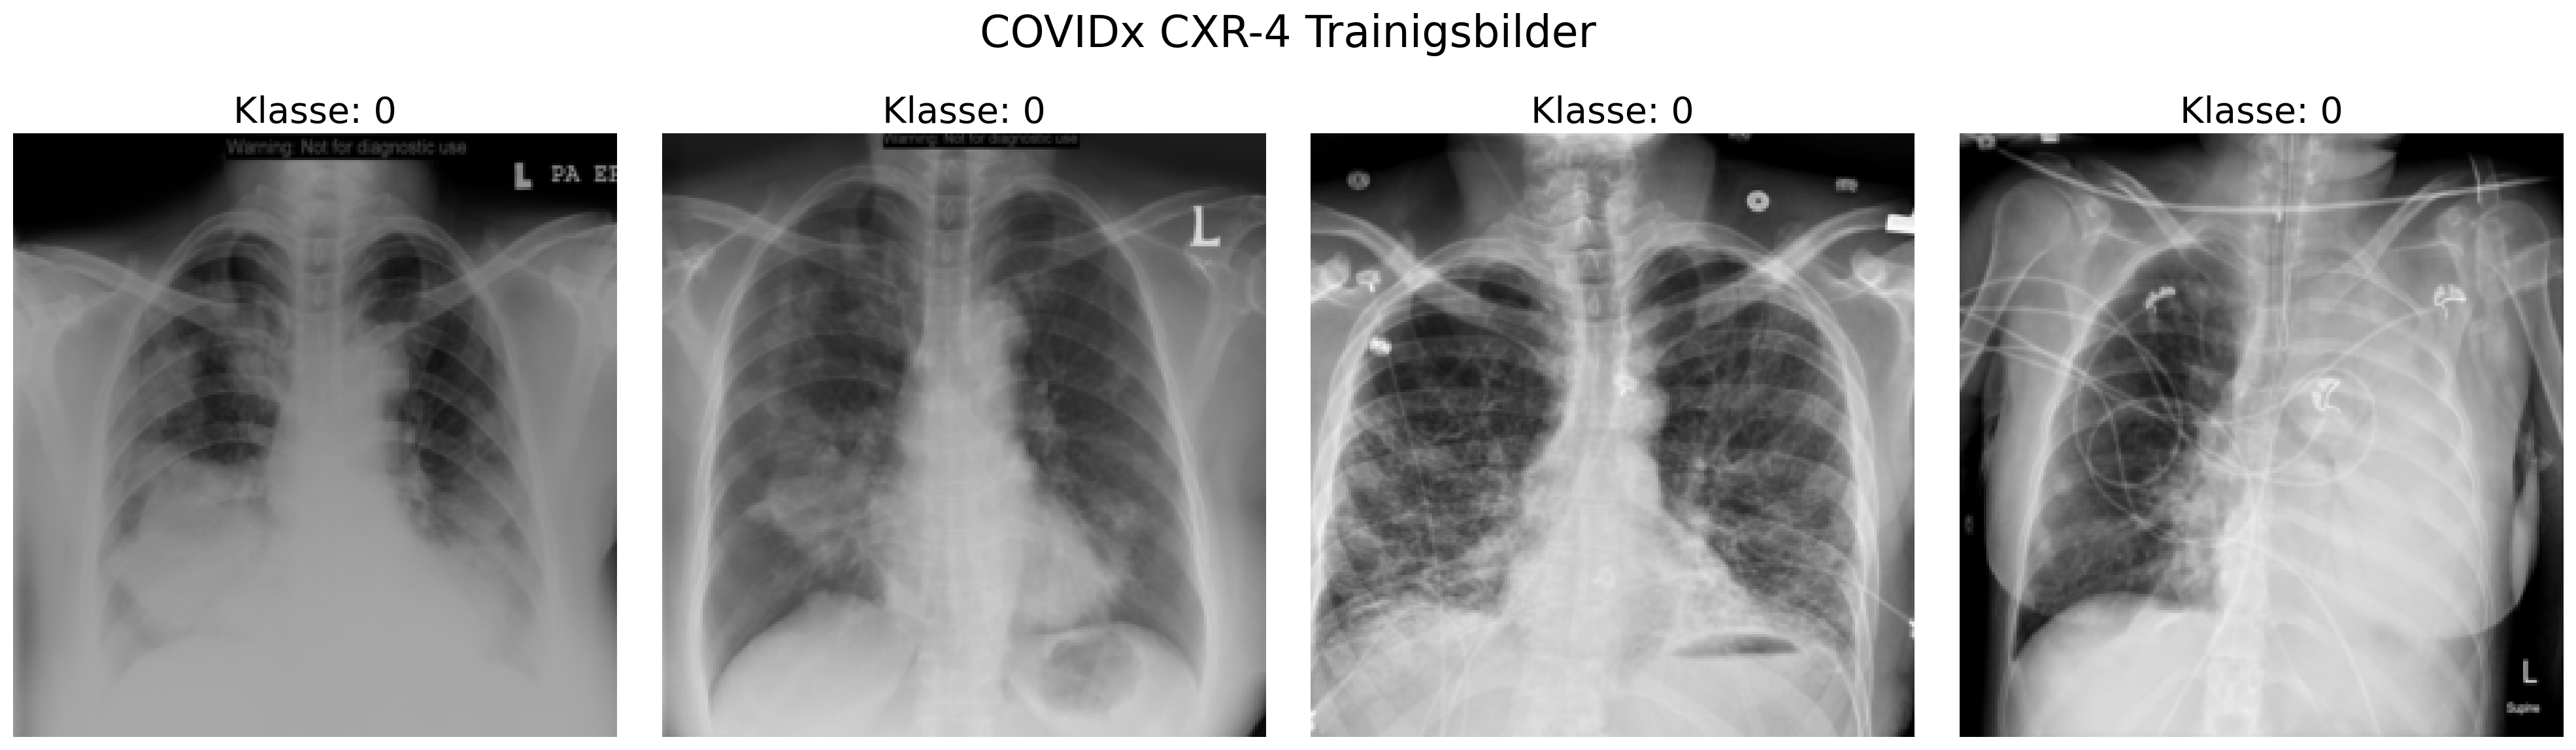
\includegraphics[width=\linewidth, height=4cm]{01-images/03-data/covid19-klasse0.png}
    \caption{Beispiele von negativen Covid Patienten vom COVIDx CXR-4 Datensatz}
    \label{fig:covid19-klasse0}
\end{figure}

\begin{figure}[H]
    \centering
    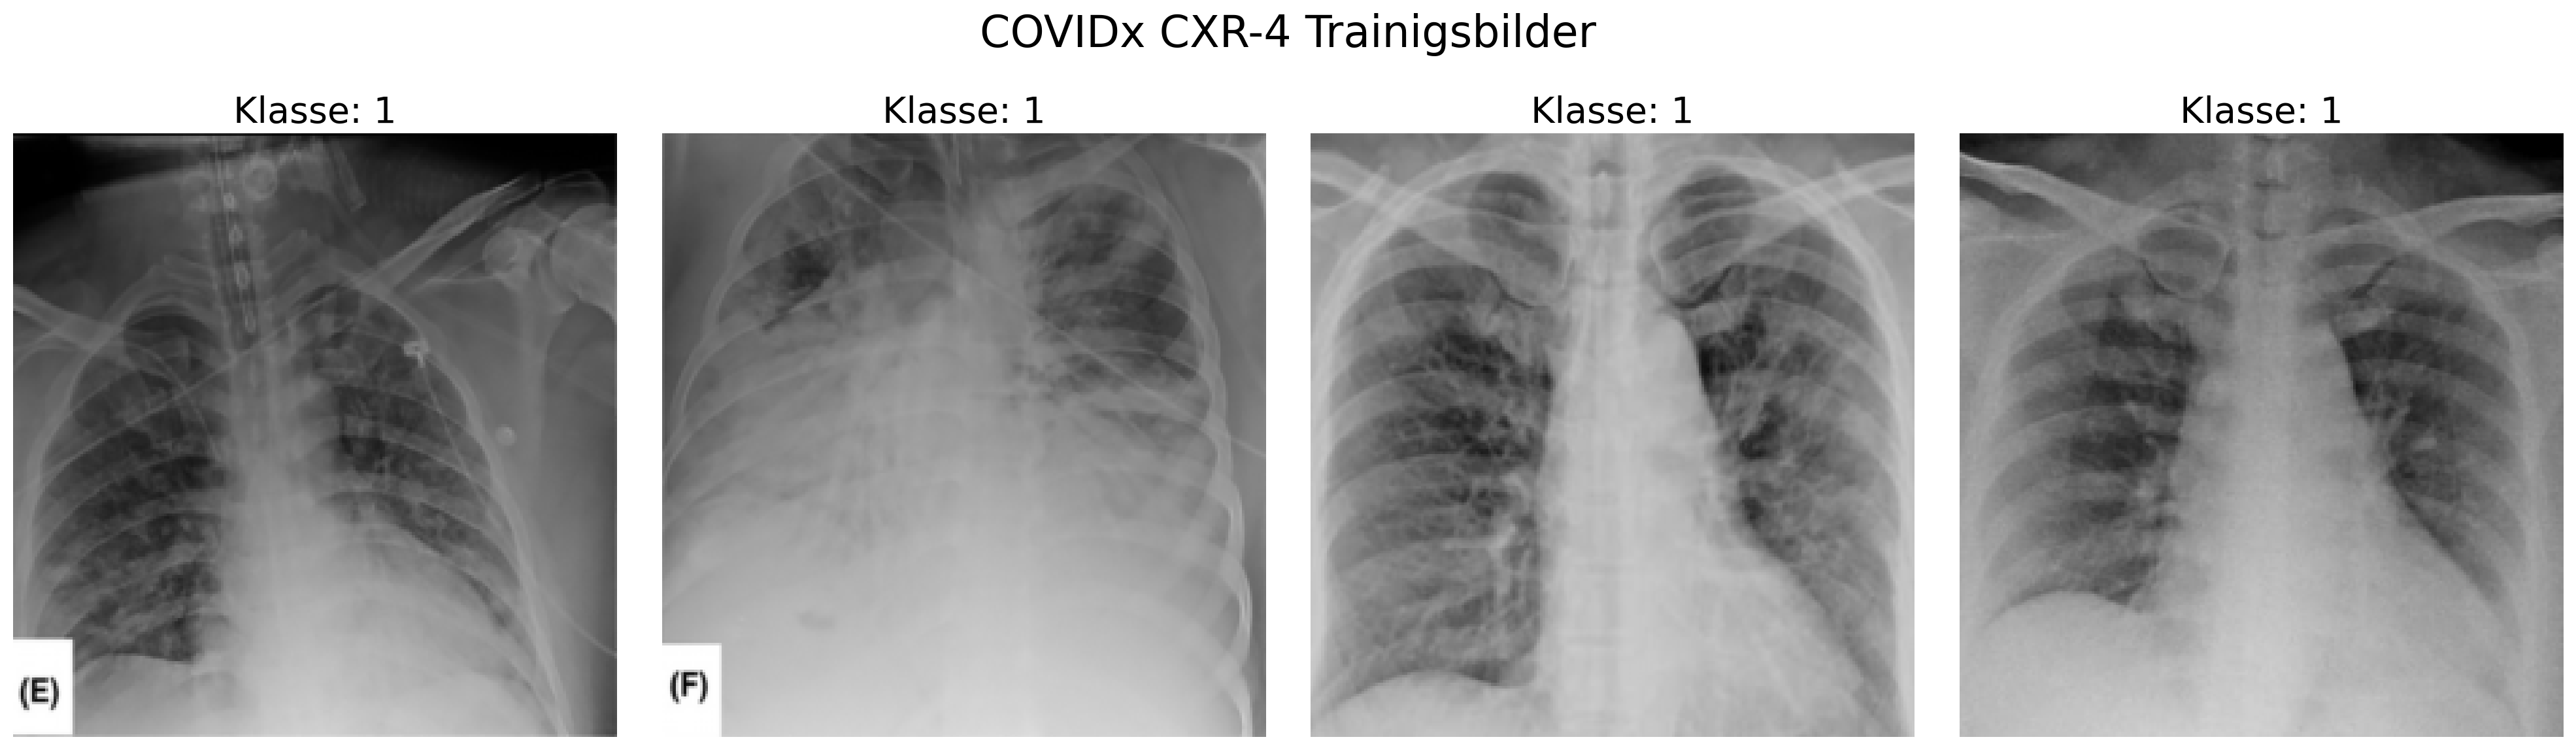
\includegraphics[width=\linewidth, height=4cm]{01-images/03-data/covid19-klasse1.png}
    \caption{Beispiele von positiven Covid Patienten vom COVIDx CXR-4 Datensatz}
    \label{fig:covid19-klasse1}
\end{figure}


\subsubsection{Datenpartitionierung} \label{chap:COVIDX-Partition}

Die Datenpartitionierung ist bereits durch die Struktur vorgegeben. Wir stellen fest, dass die Klassenverteilung von positiven und negativen Labels für die Validierung und den Testdatensets fast gleich verteilt ist, mit einem Verhältnis von 50\% positive sowie 50\% negative Fälle. 

\begin{table}[h]
\centering
\begin{tabular}{@{}cccccc@{}}
\toprule
Partition & \multicolumn{2}{c}{Anzahl Bilder} & \multicolumn{2}{c}{Klassenverteilung} & Positiv-Verhältnis\\ 
\cmidrule(lr){2-3} \cmidrule(lr){4-5} 
          & Absolut & Relativ & Positiv & Negativ & \\ 
\midrule
Train      & 67863 & 0.8001 & 57199 & 10664 & 0.8429 \\
Validation & 8473  & 0.0999 & 4241  & 4232  & 0.5005 \\
Test       & 8482  & 0.1000 & 4241  & 4241  & 0.5000 \\ 
\bottomrule
\end{tabular}
\caption{Klassenverteilung von COVIDX-CXR4}
\label{tab:covidx-klassenverteilung}
\end{table}

\subsubsection{Datenexploration}


In den dargestellten Histogrammen sehen wir die Pixelverteilung der Röntgenbilder von positiven \ref{fig:covid19-klasse1} und negativen \ref{fig:covid19-klasse0} Patienten. Jedes Histogramm repräsentiert die Intensitätsverteilung der Pixelwerte in den jeweiligen Röntgenaufnahmen. Die x-Achse jedes Histogramms zeigt die Grauwertintensität von 0 bis 255, während die y-Achse die Anzahl der Pixel für jede Intensität darstellt. 

\begin{figure}[ht]
    \centering
    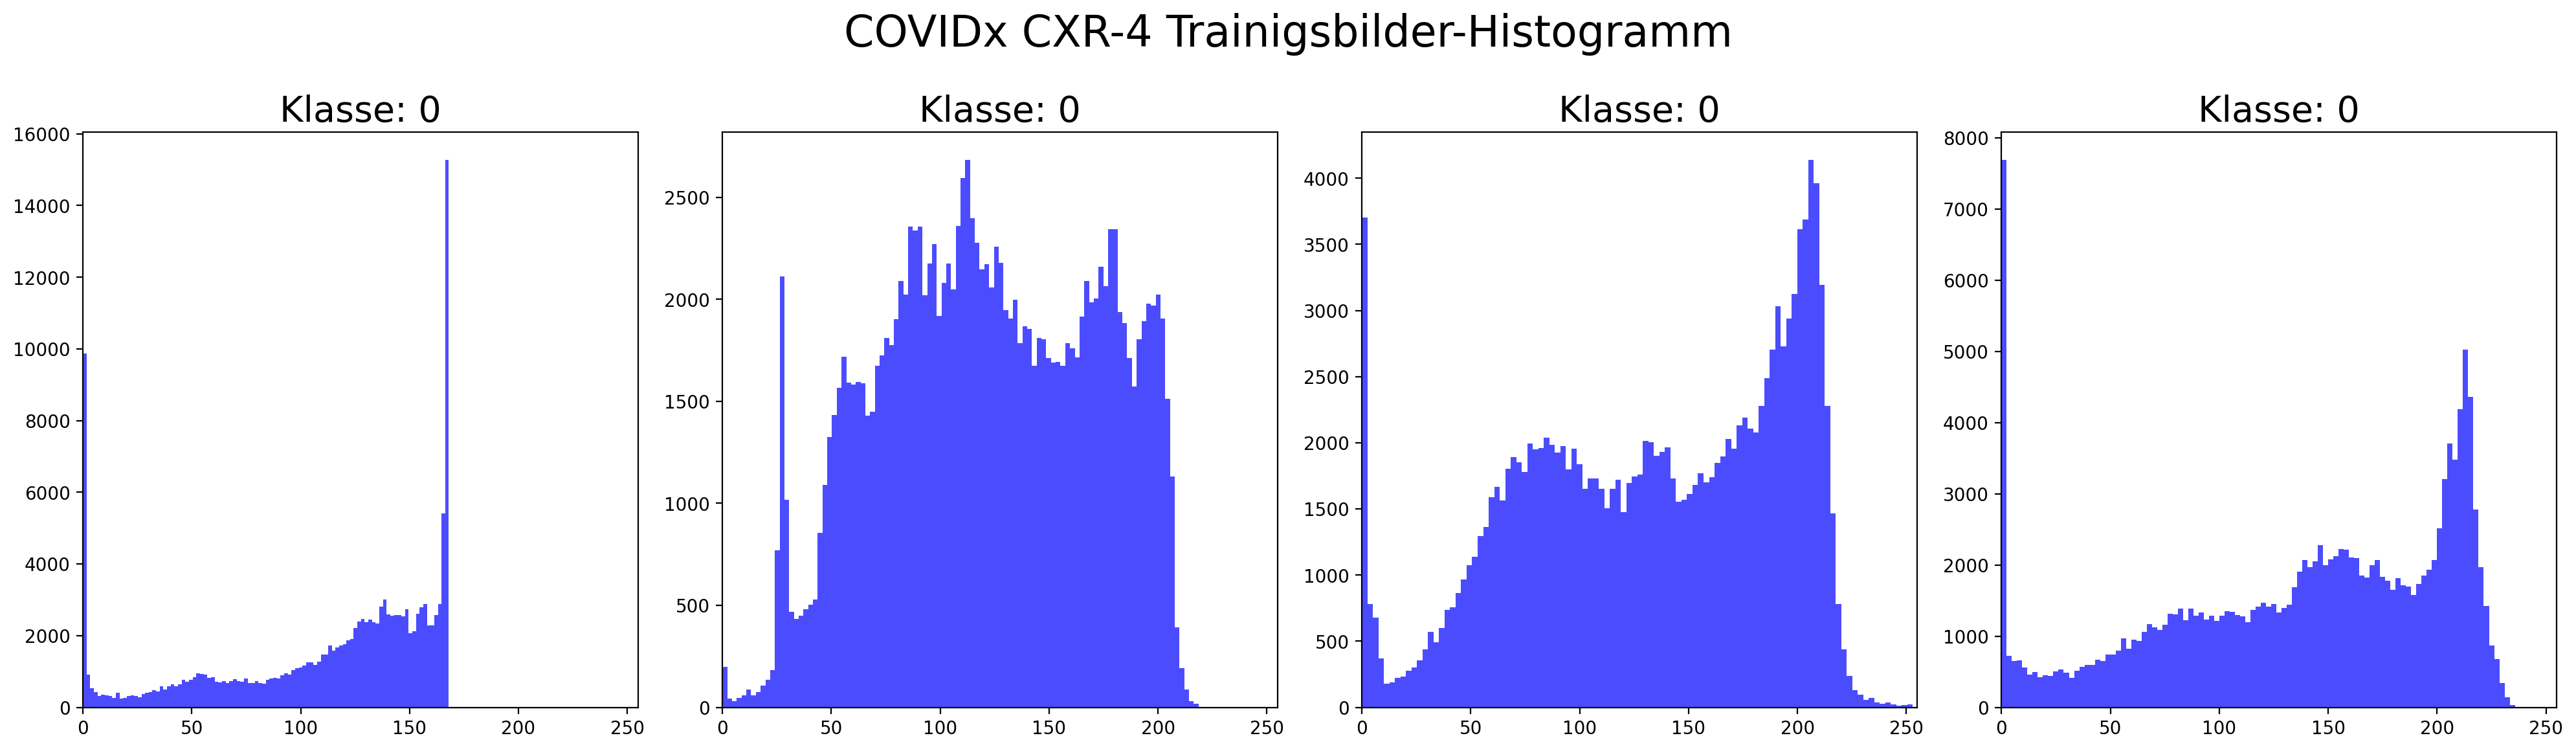
\includegraphics[width=\linewidth, height=4cm]{01-images/03-data/covid19-klasse0-hist.png}
    \caption{Histogramm der Pixelverteilung von Abbildung \ref{fig:covid19-klasse0}}
    \label{fig:covid19-klasse0-hist}
\end{figure}

\begin{figure}[ht]
    \centering
    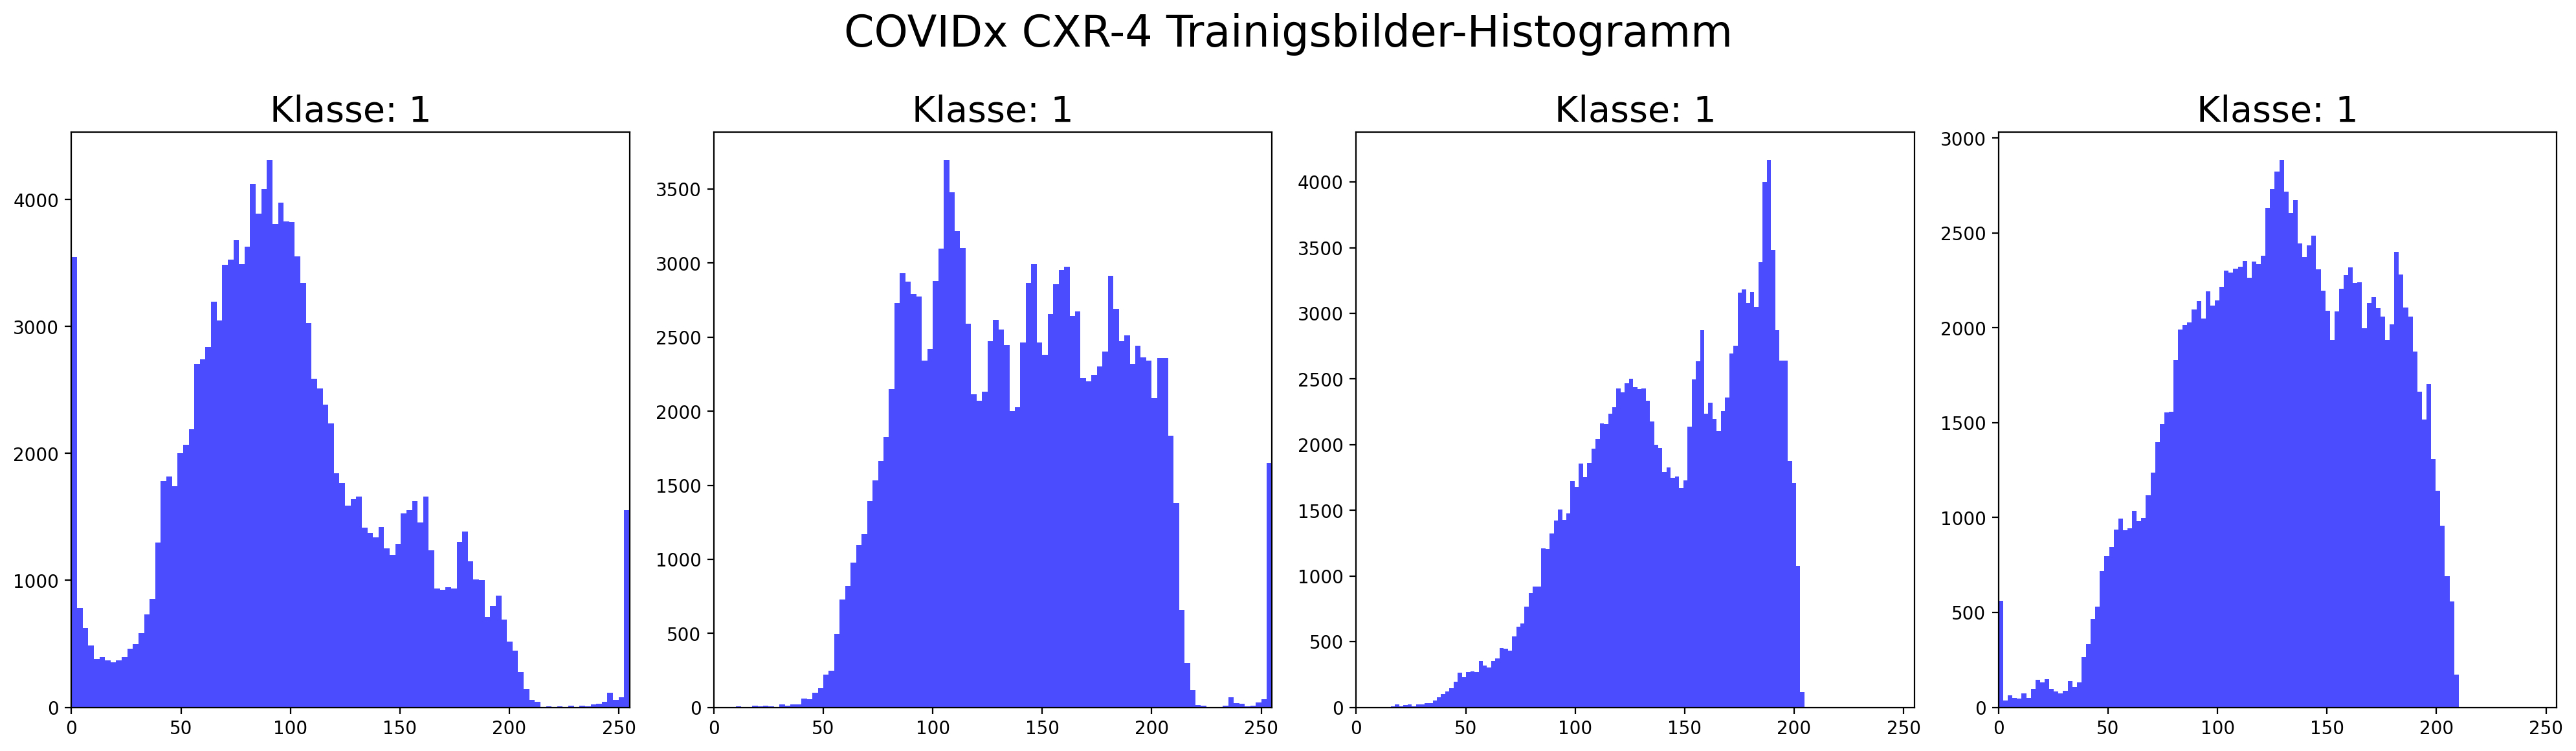
\includegraphics[width=\linewidth, height=4cm]{01-images/03-data/covid19-klasse1-hist.png}
    \caption{Histogramm der Pixelverteilung von Abbildung \ref{fig:covid19-klasse1}}
    \label{fig:covid19-klasse1-hist}
\end{figure}

Die Histogramme der Röntgenbilder variieren stark von Bild zu Bild. Tiefe Pixelwerte repräsentieren vermutlich Weichgewebe, während höhere Pixelwerte harte Knochengewebe darstellen

\newpage